\section{Результаты измерений}
\subsection{Измерение диаметра $d$ проволоки}
Измерения проводились штангенциркулем и микрометром для $N=10$ различных
участков проволоки.

\begin{table}[h!]
    \caption{Измерение диаметра проволоки штангенциркулем}
    \begin{tabular}{|l|l|l|l|l|l|l|l|l|l|l|}
    \hline
    Номер измерения             & 1       & 2       & 3       & 4       & 5       & 6       & 7       & 8       & 9       & 10      \\ \hline
    $d_{\text{шт}}$, мм         & $0{,}4$ & $0{,}4$ & $0{,}3$ & $0{,}4$ & $0{,}3$ & $0{,}4$ & $0{,}4$ & $0{,}4$ & $0{,}4$ & $0{,}4$ \\ \hline
    \end{tabular}
\end{table}
$d_{\text{шт}}=0{,}38\pm0{,}05\,\text{мм}$

$\varepsilon_d = 0{,}13$

\begin{table}[h!]
    \caption{Измерение диаметра проволоки микрометром}
    \begin{tabular}{|l|l|l|l|l|l|l|l|l|l|l|}
    \hline
    Номер измерения             & 1       & 2       & 3       & 4       & 5       & 6       & 7       & 8       & 9       & 10      \\ \hline
    $d_{\text{м}}$, мм          & $0{,}36$ & $0{,}37$ & $0{,}37$ & $0{,}35$ & $0{,}37$ & $0{,}36$ & $0{,}36$ & $0{,}37$ & $0{,}37$ & $0{,}35$ \\ \hline
    \end{tabular}
\end{table}
$d_{\text{м}}=0{,}364\pm0{,}005\,\text{мм}$

$\varepsilon_d = 0{,}013$

Измерения микрометром точнее, поэтому далее будут использоваться они.
\[S=\pi\frac{d^2}{4}=0{,}104\pm 0{,}003\,\text{мм}^2\]

\subsection{Измерение сопротивления}
Показания амперметра и вольтметра для разных длин проволоки приведены в таблице, графики изображены на рисунке.


\begin{table}[t!]
    \caption{Показания амперметра и вольтметра}
    \begin{tabular}{|llllllllllll|}
    \hline
    \multicolumn{12}{|c|}{$l=20\,\text{см}$}                                                                                                                                                                                                                                                                                                                                                         \\ \hline
    \multicolumn{1}{|l|}{$U_V$, мВ}   & \multicolumn{1}{l|}{$106{,}1$} & \multicolumn{1}{l|}{$297{,}8$} & \multicolumn{1}{l|}{$474$}      & \multicolumn{1}{l|}{$614{,}3$}  & \multicolumn{1}{l|}{$819{,}5$}  & \multicolumn{1}{l|}{$1001{,}7$} & \multicolumn{1}{l|}{$1187{,}8$} & \multicolumn{1}{l|}{$1309{,}7$} & \multicolumn{1}{l|}{$1693{,}3$} & \multicolumn{1}{l|}{$2051{,}6$} & $2436$     \\ \hline
    \multicolumn{1}{|l|}{$I_A$, мА} & \multicolumn{1}{l|}{$45$}      & \multicolumn{1}{l|}{$135$}     & \multicolumn{1}{l|}{$215$}      & \multicolumn{1}{l|}{$285$}      & \multicolumn{1}{l|}{$380$}      & \multicolumn{1}{l|}{$460$}      & \multicolumn{1}{l|}{$545$}      & \multicolumn{1}{l|}{$600$}      & \multicolumn{1}{l|}{$745$}      & \multicolumn{1}{l|}{$930$}      & $1099$     \\ \hline
    \multicolumn{12}{|c|}{$l=30\,\text{см}$}                                                                                                                                                                                                                                                                                                                                                         \\ \hline
    \multicolumn{1}{|l|}{$U_V$, мВ}   & \multicolumn{1}{l|}{$151{,}3$} & \multicolumn{1}{l|}{$360{,}3$} & \multicolumn{1}{l|}{$441$}      & \multicolumn{1}{l|}{$501{,}5$}  & \multicolumn{1}{l|}{$613$}      & \multicolumn{1}{l|}{$838{,}8$}  & \multicolumn{1}{l|}{$1009{,}5$} & \multicolumn{1}{l|}{$1207{,}4$} & \multicolumn{1}{l|}{$1504$}     & \multicolumn{1}{l|}{$1967$}     & $2314{,}5$ \\ \hline
    \multicolumn{1}{|l|}{$I_A$, мА} & \multicolumn{1}{l|}{$40$}      & \multicolumn{1}{l|}{$105$}     & \multicolumn{1}{l|}{$130$}      & \multicolumn{1}{l|}{$150$}      & \multicolumn{1}{l|}{$180$}      & \multicolumn{1}{l|}{$250$}      & \multicolumn{1}{l|}{$300$}      & \multicolumn{1}{l|}{$360$}      & \multicolumn{1}{l|}{$450$}      & \multicolumn{1}{l|}{$585$}      & $590$      \\ \hline
    \multicolumn{12}{|c|}{$l=50\,\text{см}$}                                                                                                                                                                                                                                                                                                                                                         \\ \hline
    \multicolumn{1}{|l|}{$U_V$, мВ}   & \multicolumn{1}{l|}{$347{,}3$} & \multicolumn{1}{l|}{$863{6}$}  & \multicolumn{1}{l|}{$1127{,}5$} & \multicolumn{1}{l|}{$1417{,}3$} & \multicolumn{1}{l|}{$1797{,}4$} & \multicolumn{1}{l|}{$1966{,}5$} & \multicolumn{1}{l|}{$2420{,}5$} & \multicolumn{1}{l|}{$2769$}     & \multicolumn{1}{l|}{$3175$}     & \multicolumn{1}{l|}{$3579{,}5$} & $3895$     \\ \hline
    \multicolumn{1}{|l|}{$I_A$, мА} & \multicolumn{1}{l|}{$55$}      & \multicolumn{1}{l|}{$160$}     & \multicolumn{1}{l|}{$205$}      & \multicolumn{1}{l|}{$225$}      & \multicolumn{1}{l|}{$325$}      & \multicolumn{1}{l|}{$355$}      & \multicolumn{1}{l|}{$440$}      & \multicolumn{1}{l|}{$505$}      & \multicolumn{1}{l|}{$575$}      & \multicolumn{1}{l|}{$650$}      & $705$      \\ \hline
    \end{tabular}
\end{table}

\begin{figure}[h!]
    \centering
    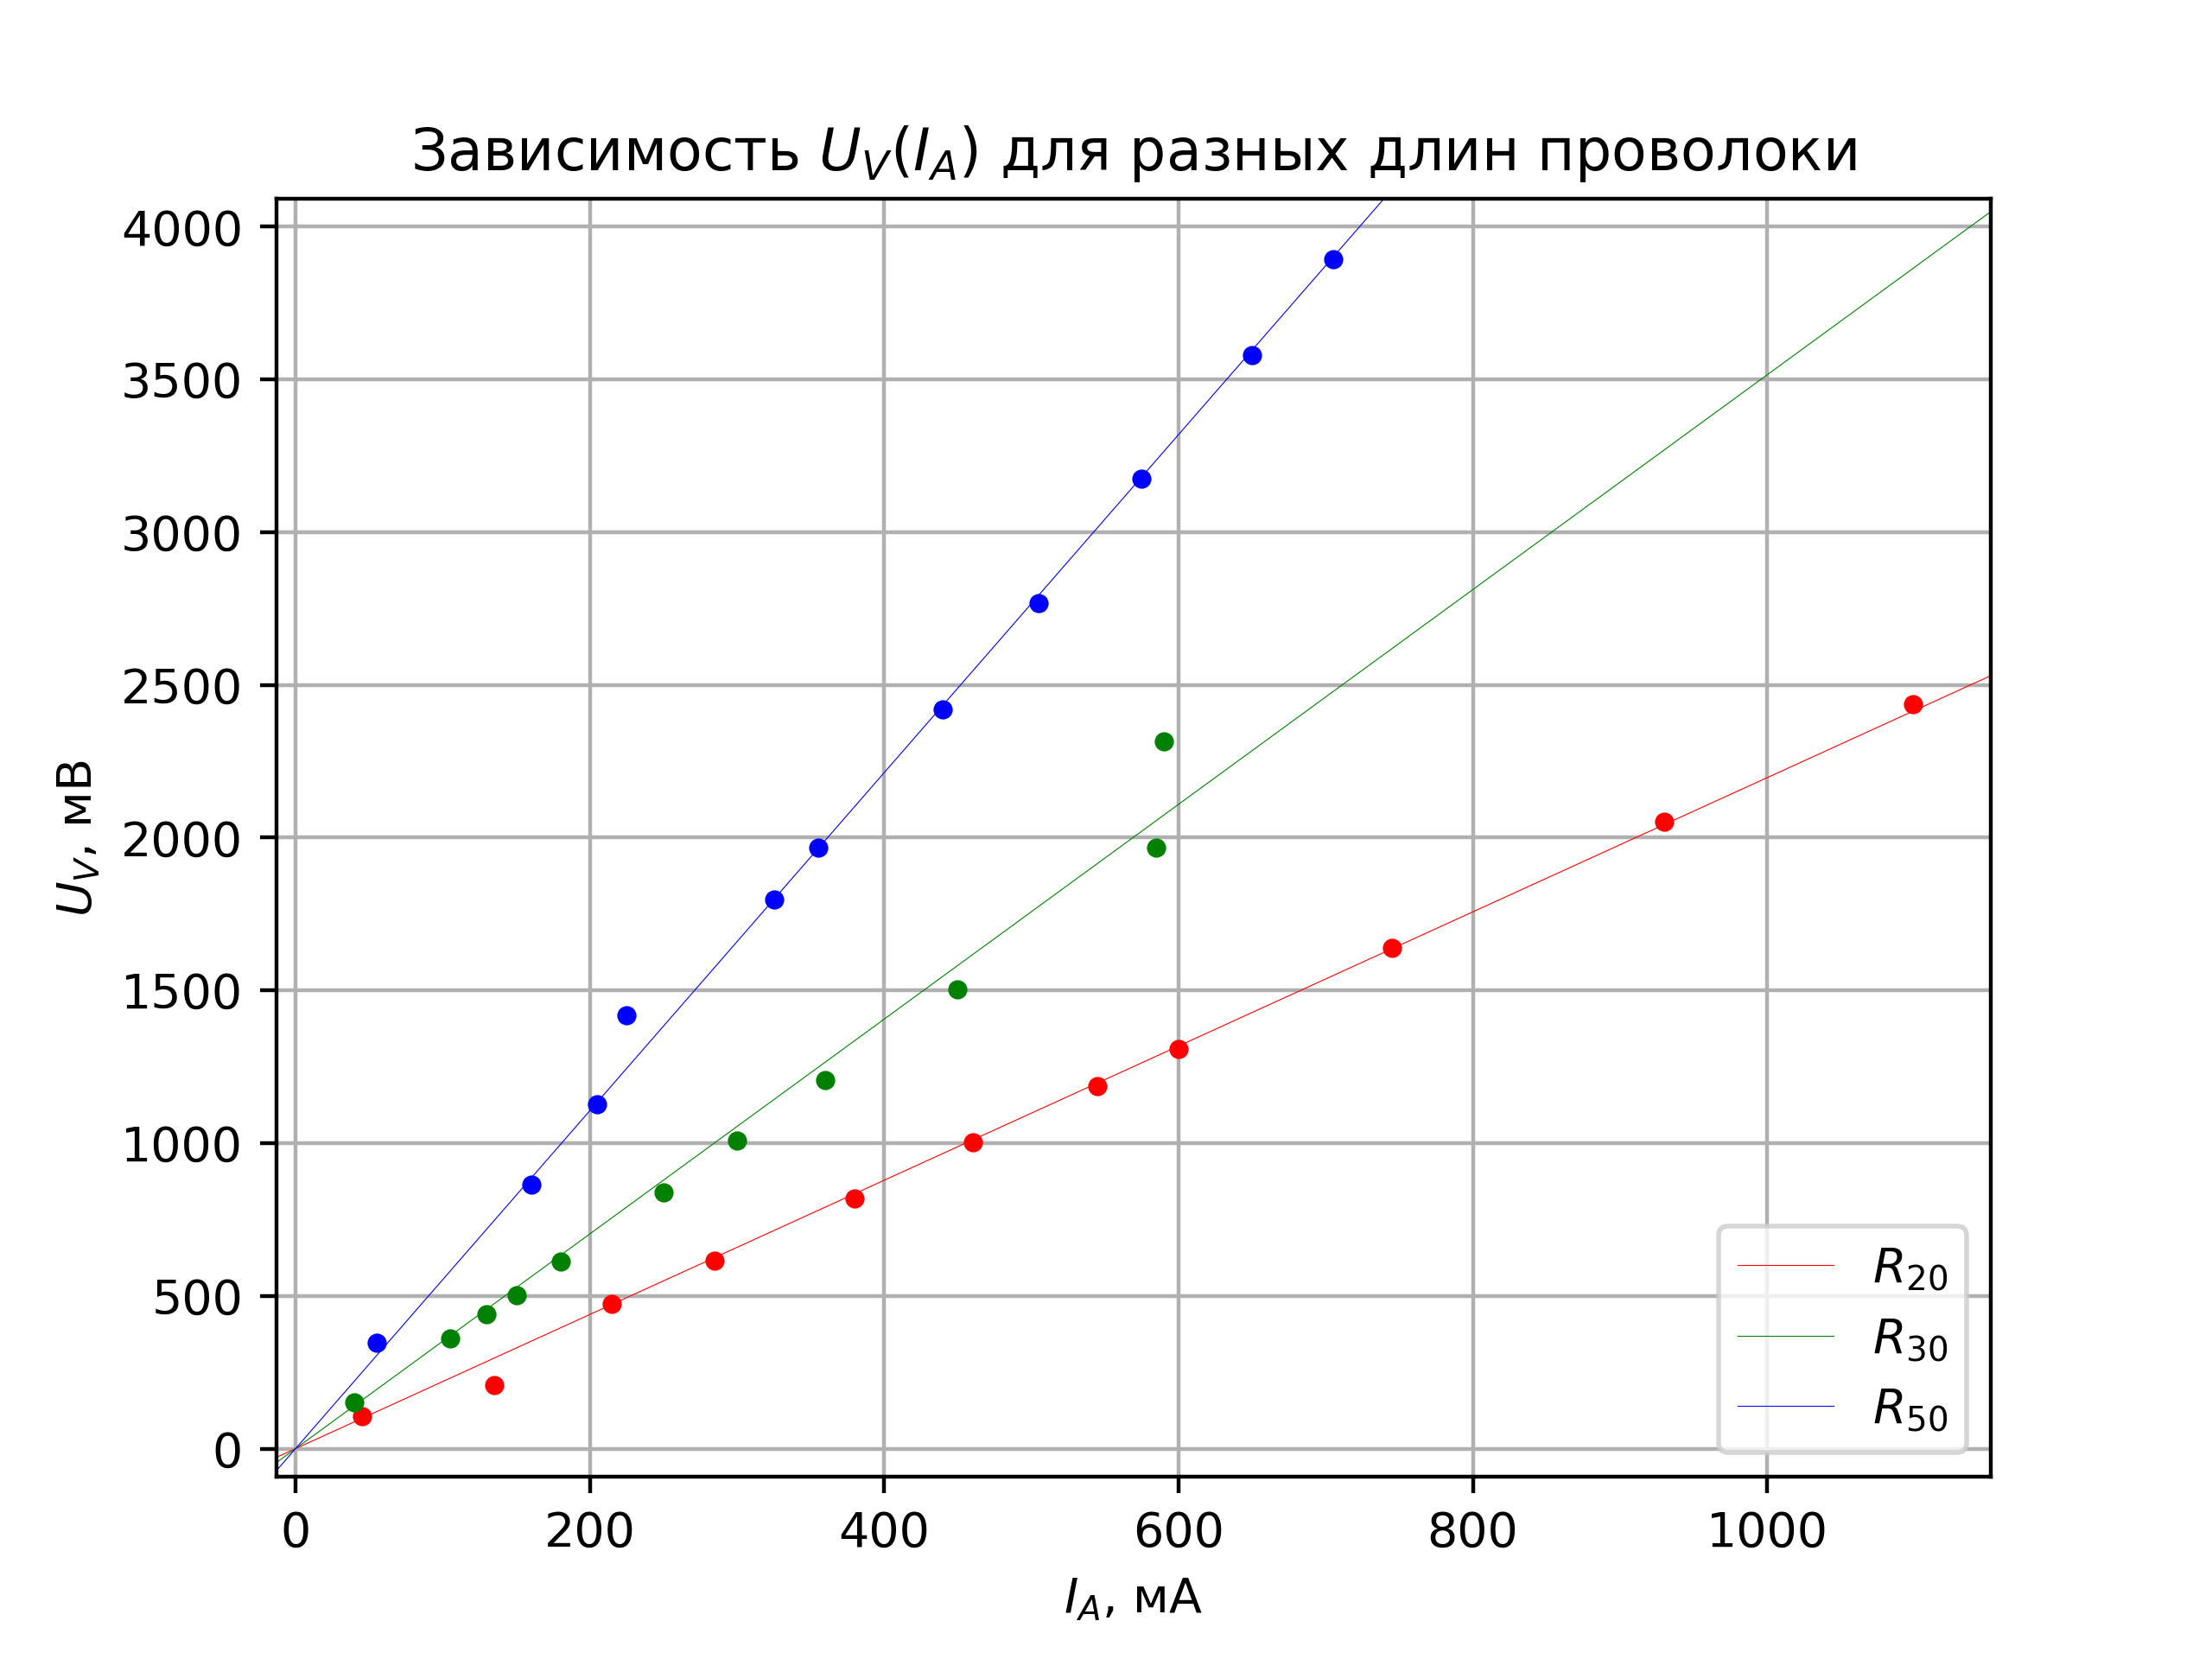
\includegraphics[width=\textwidth]{img/plot.png}
    \label{fig:circuit}
\end{figure}


По МНК находим наилуцшие значения для $R_0$:
\[\overline{R_0}=\frac{\left\langle U_VI_A\right\rangle}{\left\langle I_A^2\right\rangle}\]

Систематическая погрешность измерений будет порядка $R\frac{\Delta_{I_A}}{I_A}\sim 10^{-2}$, что на порядок меньше случайной погрешности,
поэтому систематической погрешностью можно пренебречь.

Итого:
\begin{multline*}
    \\
    R_{20}=2{,}20\pm 0{,}12\,\text{Ом}\;\;\varepsilon_{R_{20}}=0{,}05\\
    R_{30}=3{,}52\pm 0{,}12\,\text{Ом}\;\;\varepsilon_{R_{20}}=0{,}03\\
    R_{50}=5{,}53\pm 0{,}15\,\text{Ом}\;\;\varepsilon_{R_{20}}=0{,}03\\
\end{multline*}

Измерения при помощи моста дают следующие результаты:
\begin{multline*}
    \\
    R_{20}=2{,}169\pm 0{,}01\,\text{Ом}\;\;\varepsilon_{R_{20}}=0{,}005\\
    R_{30}=3{,}305\pm 0{,}01\,\text{Ом}\;\;\varepsilon_{R_{20}}=0{,}003\\
    R_{50}=5{,}4301\pm 0{,}01\,\text{Ом}\;\;\varepsilon_{R_{20}}=0{,}002\\
\end{multline*}

Значения $R_{20}$ и $R_{50}$, измеренные при помощи графика, отличаются от соответствующих значений для моста,
но лежат в пределах погрешностей. А вот $R_{30}$ довольно сильно отличается от значения, данного мостом. Это
может быть связано с выбросным последним измерением. если его не учитывать, то $R_{30}=3{,}36\pm0{,}11\,\text{Ом}$,
что совпадает со значением моста в пределах погрешности.

Далее будут использоваться значения $R_0$ для моста, т.к. они дают меньшую погрешность.
\begin{multline*}
    \\
    \rho_{20}=\left(1{,}13\pm 0{,}03\right)\cdot 10^{-6}\,\text{Ом}\cdot\text{м}\\
    \rho_{30}=\left(1{,}15\pm 0{,}03\right)\cdot 10^{-6}\,\text{Ом}\cdot\text{м}\\
    \rho_{50}=\left(1{,}13\pm 0{,}03\right)\cdot 10^{-6}\,\text{Ом}\cdot\text{м}\\
\end{multline*}
Окончательно $\rho=\left(1{,}14\pm 0{,}03\right)\cdot 10^{-6}\,\text{Ом}\cdot\text{м}$ лежит в пределах допустимых значений.

Измерения $l$ дают относительную погрешность $\varepsilon_l=10^{-3}$. При достигнутых точностях измерений $l$ и $d$ сопротивление можно
измерять с точностью не более, чем $2\cdot\varepsilon_d/2\approx0{,}01$.

\section{Вывод}
Значения $\rho$ лежат в пределах допустимых (от $1{,}05$ до $1{4}\,\text{Ом}\cdot\text{м}$), точность измерений довольно высока (порядка $1\,\%$). Наибольший вклад в погрешность вносит
точность измерения диаметра проволоки.
